% 
%% SOSP 2017 Template
%%
%% Uses sigplanconf from:
%% 
%%    http://www.sigplan.org/sites/default/files/sigplanconf.cls
%%
%% with 10pt and preprint options. 
%%
%% Replace 'XX' with your paper number (assigned when you register abstract)
%% Replace 'NN' with actual number of pages. 

\documentclass[10pt,preprint]{sigplanconf}
\usepackage{times}

\usepackage{datetime}
\usepackage{url}
\usepackage{hyperref}
\usepackage{graphicx}

\conferenceinfo{SOSP'17}{October 29--31, 2017, Shanghai, China}
\copyrightyear{2017} 


% These only appear when the 'preprint' option is specified.
% Enabling these will cause the first page of the document to fail the 
% format check on HotCRP :-(
%\titlebanner{Under submission to SOSP 2017 - do not cite or distribute}
%\preprintfooter{Draft of {\currenttime}, \today{}}

% No date in title area.
\date{}

% Paper number and no. of pages as author
\authorinfo{Keyan Chen(kc32),  Zhiyuan Tang(zt6)}{8 pages}


% Actual document begins below.
\begin{document}

\title{Generic Mutex Subsystem of Linux Kernel} 
\maketitle

\begin{abstract}

Sample abstract.

\end{abstract}

\section{Breif History and Background}

In the linux kernel, mutexes refer to a particular locking primitive that enforces serialization on shared memory systems, and not only to the generic term referring to ‘mutual exclusion’ found in academia or similar theoretical textbooks. \\\\
Before 2006, when developers wanted to gain mutual exclusion among their shared memory systems, they would use binary semaphores, which are sleeping locks. However, Mutexes were introduced in 2006 as an alternative to binary semaphores and this new data structure provided a number of advantages, including simpler interfaces, and at that time smaller code. 

\subsection{Why Mutex?}
Why do we need a new mutex subsystem? And what's wrong with semaphores?\\
\begin{enumerate}
	\item 'struct mutex' is smaller.
	\begin{enumerate}
		\item On x86, 'struct semaphore' is 20 bytes, 'struct mutex' is 16 bytes. A smaller structure size means less RAM footprint, and better CPU-cache utilization
	\end{enumerate}
	\item Mutex can result in tighter code
	\begin{enumerate}
		\item On x86 we can get the following .text sizes when switching all mutex-alike semaphores in the kernel to the mutex subsystem
		\begin{figure}[h!]
			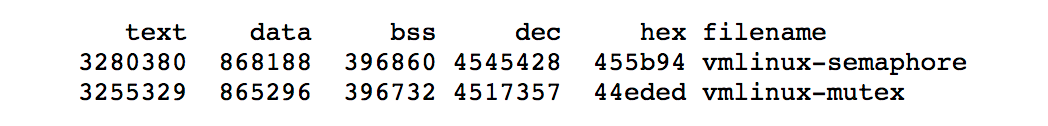
\includegraphics[scale=0.5]{image00.png}
		\end{figure}
		\item That's 25021 bytes of code saves, or a 0.76\% win off the hottest codes paths of the kernel
		\item Smaller code means better in-cache footprint, which is one of the major optimization goals in the linux kernel when people were proposing the addition of mutex subsystem in 2006. 
	\end{enumerate}
	\item The mutex subsystem is faster and has superior scalability for contented workloads.
	\begin{enumerate}
		\item On a 8-way x86 system, running a mutex based kernel and testing create+unlink+close(of separate, per-task files) in /tmp with 16 parallel tasks, the average number of ops/sec is 
		\begin{figure}[h!]
			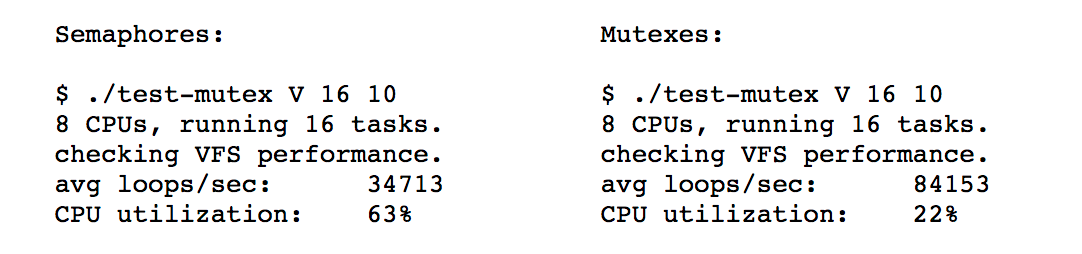
\includegraphics[scale=0.55]{image01.png}
		\end{figure}
		\item In this workload, mutex based kernel was \textbf{2.4 times} faster than the semaphore based kernel, and it also had \textbf{2.8 times} less CPU utilization. 
	\end{enumerate}
\end{enumerate}


\subsection{Design and Implementation details}
Mutex is represented by ‘struct mutex’, defined in include/linux/mutex.h and implemented in kernel/locking/mutex.c. The mutex uses a three state atomic counter to represent the different possible transitions that can occur during the lifetime of a mutex:
\begin{itemize}
	\item 1: unlocked
	\item 0: locked, no waiters
	\item negative: locked, with potential waiters
\end{itemize}
In its most basic form it also includes a wait-queue and a spinlock that serializes access to it. When acquring a mutex, there are three possible paths that can be taken, depending on the state of lock:
\begin{enumerate}
	\item Fastpath: tries to atomically acquire the lock by decrementing the counter. If it was already taken by another task it goes to the next possible path. This logic is architecture specific.
	\item Mid-path: aka optimistic spinning. It tries to spin for acquisition while the lock owner is running and there are no other tasks ready to run that have higher priority. The rationale is that if the lock owner is running, it is likely to release the lock soon. The mutex spinners are queued up using MCS lock so that only one spinner can compete for the mutex. The MCS lock is a simple spinlock with the desirable properties of being fair and with each cpu trying to acquire the lock spinning on a local variable. It avoids expensive cache-line bouncing that common test-and-set spinlock implementations incur. And MCS-like lock is specially tailored for optimistic spinning for sleeping lock implementation.
	\item Slowpath: last resort, if the lock is still unable to be acquired, the task is added to the wait-queue and sleeps until woken up by the unlock path. Under normal circumstances it blocks as TASK\_UNINTERRUPTIBLE.
\end{enumerate}

\section{Interesting Findings}
\subsection{Unique Optimistic Spinning in Linux Mutex Subsystem}
While formally kernel mutexes are sleepable locks, it is the Mid-path(aka optimistic spinning) that makes the mutex subsystem now more practically a hybrid type. By simply not interrupting a task and busy-waiting for a few cycles instead of immediately sleeping, the performance of this lock has been seen to significantly improve a number of workloads. \\

\begin{figure}[h!]
	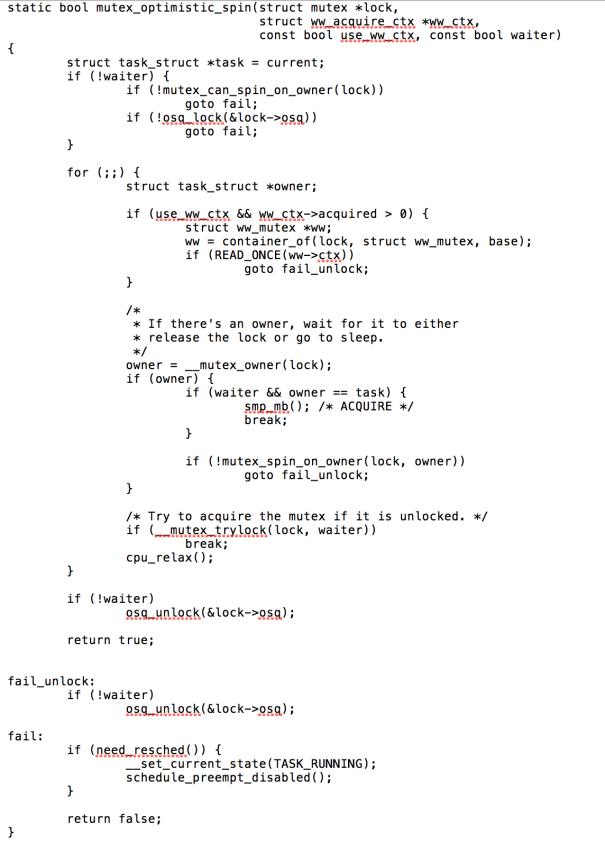
\includegraphics[scale=1]{image02.png}
	\caption{Use of MCS and the Optimistic Spinning routine in the source code}
\end{figure}


\subsection{Use of MCS lock in linux kernel}
In mutex subsystem, mutex spinners are queued up using MCS locks as talked about above. 
The design of MCS lock and the difference between MCS lock and ordinary spinlock is also a very interesting design decision in linux kernel.\\
The concept of a spinlock is simple and straight-forward. When a thread wants to acquire the lock it will attempt to set the lock bit of that spinlock with an atomic compare-and-swap(CAS) instruction and repeatedly spin there in the lock can not be acquired during one CAS. \\
However, spinlocks have some fundamental problems. One of those is that every attemp to acquire a lock requires moving the cache line containing that lock to the local CPU. This cache-line bouncing can be extremely bad to performance for contended locks. Therefore, developers had been working on reducing the cache contention of spinlocks and thus, MCS locks were introduced by Tim Chen to solve this problem.


\subsection{Bug in an obviously correct reference count code pattern}



\bibliographystyle{acm}
% \bibliography{xxx}

\end{document}
